\section{\textit{A Priori} Analysis}
\label{sec:subfilter:dns}

\subsection{DNS Database}
\label{sec:subfilter:dns:database}

The accuracy of the proposed $Z$-Activated Soot Subfilter PDF is validated through an \textit{a priori} analysis using the database from a three-dimensional DNS of a temporally evolving, turbulent nonpremixed planar jet flame at atmospheric pressure~\cite{attili2014}. In this simulation, a central fuel slab consisting of a \textit{n}-heptane/nitrogen [15/85 by volume] mixture at 400 K is surrounded on either side by an air coflow at 800 K. The initial velocity field of the fuel jet is obtained from an instantaneous realization of a turbulent channel flow at $Re_{\tau} = 390$ with a centerline value of $U_c = 8.74$ m/s. The surrounding air flows in the opposite direction of the fuel jet with a streamwise velocity of the same magnitude to give a jet Reynolds number $Re = 2U_c H/\nu \approx 15,000$.

Oxidation of \textit{n}-heptane is modeled with a reduced mechanism comprising 47 species and 290 reactions that accounts for the formation of PAH up to naphthalene. The soot model, as described in \cref{ch:lesmodels,ch:subfilter}, is used in both the DNS and the \textit{a priori} analysis. In the DNS, the soot population is described with seven statistical moments, whereas only three moments and the weight of the delta function are used in the \textit{a priori} investigation. The choice to use a reduced set of moments allows for validation of the proposed soot model with parameters that will most likely be implemented in LES.

The DNS domain is discretized with $N_x \times N_y \times N_z = 1024 \times 1024 \times 512$ grid points, where the homogeneous region of the domain ($|y/H| \le 2.8$) has a grid spacing of $h = 91\ \mu$m. For a filter width $\Delta$, the \textit{a priori} study utilizes a subset of the domain of size $N_x \times N_y \times (\Delta/h + 1)$, where low-pass filtering is done only within the homogeneous mesh region. As shown in the subsequent analysis, this provided sufficiently smooth statistics. Analysis is performed on a snapshot of the DNS at $t = 5$ ms. Other key properties of the DNS are summarized in \cref{tab:subfilter:dns:params} and complete details can be found in Attili \etal~\cite{attili2014}.

\begin{table}[htbp]
\centering
\caption[Parameters for DNS of Turbulent Nonpremixed \ce{C7H16}/\ce{N2} Jet Flame]{Parameters for DNS of a turbulent nonpremixed \ce{C7H16}/\ce{N2} jet flame~\cite{attili2014}}
\label{tab:subfilter:dns:params}
\begin{tabular}{p{0.46\textwidth} p{0.15\textwidth} p{0.2\textwidth}}
\toprule
Initial jet width, $H$
& [mm] & 15 \\[0.2em]

Domain size, $L_x \times L_y \times L_z$
& [mm] & $94 \times 105 \times 47$ \\[0.2em]

Time step, $\Delta t$
& [$\mu$s] & 4 \\[0.2em]

Minimum Kolmogorov scale, $\eta$
& [$\mu$m] & 110 \\[0.2em]

Kinematic viscosity of fuel mixture, $\nu$
& [m$^2$s$^{-1}$] & $1.7 \times 10^{-5}$ \\[0.2em]

Stoichiometric mixture fraction, $Z_{st}$
& [--] & 0.147 \\

\bottomrule
\end{tabular}
\end{table}

In order to validate the proposed LES model against DNS, a low-pass filter must be applied to the chosen snapshot of the DNS database. A three-dimensional, clipped and renormalized Gaussian filter kernel is employed and is given by
\begin{equation}\label{eq:subfilter:dns:kernel}
  F(x,y,z) = \kappa^3\exp\left[ \frac{-6(x^2 + y^2 + z^2)}{\Delta^2} \right],
\end{equation}
where $\Delta$ is the filter width and $\kappa$ is a renormalization constant that ensures the following relation holds for a grid spacing $h$:
\begin{equation}\label{eq:subfilter:dns:unity}
  \sum\limits_{x = -\Delta/2h}^{\Delta/2h} \sum\limits_{y = -\Delta/2h}^{\Delta/2h} \sum\limits_{z = -\Delta/2h}^{\Delta/2h} F(x,y,z) = 1.
\end{equation}
The above relations require a homogeneous mesh such that $\kappa = \kappa_j$, $\Delta = \Delta_j$, and $h = h_j$, where the index $j \in \{ x,y,z \}$. As evident in \cref{eq:subfilter:dns:unity}, the filter kernel is active over a cube of $(\Delta/h + 1)^3$ grid points. 

In the following subsections, the filtered moment source terms for oxidation and surface growth will be evaluated with the soot subfilter PDFs of \cref{sec:subfilter:zussp,sec:subfilter:zassp}. Expressions for the oxidation source terms are given by \cref{eq:subfilter:zussp:ox,eq:subfilter:zassp:ox}, and the source terms for surface growth take analogous forms. Analysis of the filtered moment source term for oxidation is considered first.

\subsection{Oxidation Source Term}
\label{sec:subfilter:dns:ox}

The following study will focus on the contribution of the filtered moment source term for oxidation to the total volume fraction, $\fst[M]{1,0}^{ox}$. Oxidation occurs at the surface of soot particles, so the expression for the source term depends on the filtered moment for the total soot surface area $\mean{M}_{0,1}$. Several approximations need to be made with regards to \cref{eq:subfilter:zassp:ox} before the \textit{a priori} analysis can be performed. First, the oxidation coefficient $k_{ox}(Z)$ is not present in the DNS database because quantities in the database are not expressed as functions of the mixture fraction as in the nonpremixed flamelet model utilized for LES. Therefore, $k_{ox}(Z)$ will be taken with a density-weighted conditional average from the DNS data
\begin{equation}\label{eq:subfilter:dns:condkox}
  \begin{split}
    k_{ox}(Z) &\approx \{ k_{ox}(x_j)|Z(x_j) \} \\
    &= \frac{<\rho(x_j)k_{ox}(x_j)|Z(x_j)>}{<\rho(x_j)|Z(x_j)>},
  \end{split}
\end{equation}
where the angle brackets $< \cdot >$ denote the conditional averaging operator and the curly brackets $\{ \cdot \}$ denote the density-weighted conditional averaging operator. This quantity is plotted in \cref{fig:subfilter:dns:kox}, where it is evident that the oxidation coefficient at mixture fractions $Z < 0.1$ and $Z > 0.4$ is well-approximated by \cref{eq:subfilter:dns:condkox}. There is some scatter in the DNS field at $0.1 < Z < 0.4$, indicating that additional conditional averaging against the scalar dissipation rate or another variable could be performed for a more accurate approximation. However, the focus here is on validating the proposed subfilter PDF, not on modeling the oxidation rate coefficient.

\begin{figure}[htb]
  \centering
  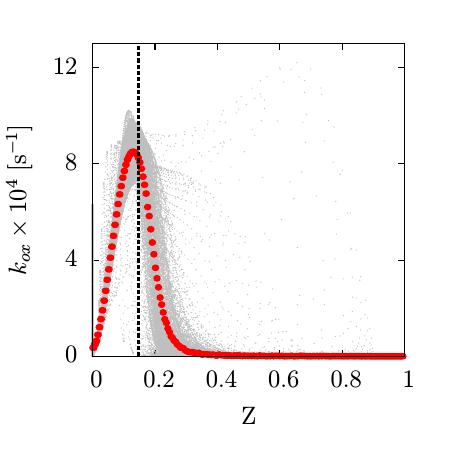
\includegraphics[width=0.43\linewidth]{ch-subfiltermodeling/figures/koxvsz}
  \caption[Approximation for Oxidation Coefficient, $k_{ox}(Z)$]{Density-weighted, conditionally averaged approximation for the oxidation coefficient $k_{ox}(Z)$. The gray dots represent $k_{ox}(x_j)|Z(x_j)$ from DNS and the red circles are the approximation $\{ k_{ox}(x_j)|Z(x_j) \}$, evaluated with 200 bins. The vertical black dashed line marks the location of stoichiometric mixture fraction $Z_{st} = 0.147$.}
  \label{fig:subfilter:dns:kox}
\end{figure}

The second quantity that needs to be estimated is the subfilter PDF for mixture fraction $\pz$, since the DNS database does not have the infinite number of points required to construct the true statistical distribution. As before, this work will presume the form of a beta distribution for $\pz$. The error associated with this assumption can be discerned by juxtaposing two versions of \cref{eq:subfilter:zussp:ox} that use the same $Z$-Uniform Soot Subfilter PDF, but approximate $k_{ox}(Z)$ with and without $\pz$. The form of the filtered moment source term for oxidation that excludes $\pz$ shall be referred to as the ``ZUSSP without $\pz$'' case and is given by
\begin{equation}\label{eq:subfilter:dns:mzusspwithoutpz}
  \fst[M]{1,0}^{ox} = \tf{k}_{ox}(Z(x_j)) \cdot \mean{M_{0,1}(x_j)},
  % \fst[M]{1,0}^{ox} = \{ \tf{k_{ox}(x_j)|Z(x_j)} \} \cdot \mean{M_{0,1}(x_j)}.
\end{equation}
where $k_{ox}(Z(x_j))$ provides the value of the oxidation coefficient at $x_j$ through \cref{eq:subfilter:dns:condkox}. $\tf{k}_{ox}(Z(x_j))$ is the result of Favre filtering the field given by the latter.

%describes the field where the value of the oxidation coefficient at $x_j$ is given by \cref{eq:subfilter:dns:condkox} based on $Z(x_j)$. $\tf{k}_{ox}(Z(x_j))$ is the result of Favre filtering the latter.
%Use of the $Z$-uniform soot subfilter PDF implies that the soot scalars are assumed to be independent of the thermochemical variables. This property is evident in \cref{eq:subfilter:dns:mzusspwithoutpz}, where the two components are distinctly separated.

The source term using $\pz$ will be referred to as the ``ZUSSP with $\pz$'' case, and is given by
\begin{equation}\label{eq:subfilter:dns:mzusspwithpz}
  \fst[M]{1,0}^{ox} = \int\limits_0^1 \{ k_{ox}(x_j)|Z(x_j) \}\tf{P}(Z; \tf{Z}(x_j),\tf{Z_V}(x_j)) dZ \cdot \mean{M_{0,1}(x_j)}.
  % \fst[M]{1,0}^{ox} = \int\limits_0^1 \{ k_{ox}|Z \}\tf{P}(Z; \tf{Z}(x_j),\tf{Z_V}(x_j)) dZ \cdot \mean{M_{0,1}(x_j)},
\end{equation}
%where $\{ k_{ox}|Z \}$ is the density-weighted, conditionally averaged oxidation coefficient as given in \cref{eq:subfilter:dns:condkox}.
\Cref{eq:subfilter:dns:mzusspwithoutpz,eq:subfilter:dns:mzusspwithpz} are first individually compared to the filtered moment source term from DNS, which will be referred to as the ``DNS'' case, and is given by
\begin{equation}\label{eq:subfilter:dns:mdns}
  \fst[M]{1,0}^{ox} = \mean{ k_{ox}(Z(x_j)) \cdot M_{0,1}(x_j)}.
  % \fst[M]{1,0}^{ox} = \mean{\{ k_{ox}(x_j)|Z(x_j)\} \cdot M_{0,1}(x_j)}.
\end{equation}
These comparisons are visible for a normalized filter width of $\Delta/h = 32$ in \cref{fig:subfilter:dns:erroronbetaox}. The top two plots show that \cref{eq:subfilter:dns:mzusspwithoutpz,eq:subfilter:dns:mzusspwithpz} generally overpredict the oxidation rate compared to the value from DNS. However, when they are compared with each other in the bottom left plot, the sample standard deviation $\sigma$ is roughly an order of magnitude smaller. This suggests that the error associated with presuming the form of a beta distribution for $\pz$ is much less than the error associated with using the $Z$-Uniform Soot Subfilter PDF to evaluate the filtered moment source term for oxidation.

The validity of presuming the beta distribution is more easily elucidated in the bottom right plot of \cref{fig:subfilter:dns:erroronbetaox}, where the cumulative distribution function (CDF) is plotted for $\fst[M]{1,0}^{ox}$. It can be observed that the distance between the lines representing \cref{eq:subfilter:dns:mzusspwithoutpz,eq:subfilter:dns:mzusspwithpz} is generally much less than the deviation between the latter and the source term from DNS at a fixed $\fst[M]{1,0}^{ox}$. These trends hold true for larger filter widths as well. % This trend is not valid when the magnitude of the source term is on the order of $10^2$ to $10^3$, where the error of presuming a beta distribution is commensurate with the error from the form of the soot subfilter PDF. Nevertheless, the most important values of the source term are the largest, where the error associated with presuming the form of a beta distribution for $\pz$ is relatively small.

\begin{figure}[ht]
  \centering
  \begin{subfigure}[b]{0.375\linewidth}
    \centering
    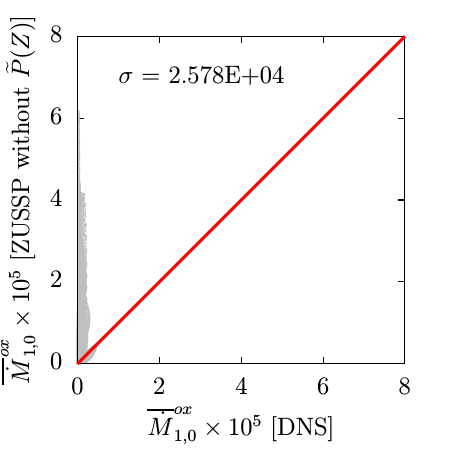
\includegraphics[width=\linewidth]{ch-subfiltermodeling/figures/lin-Mox3vsMox6-r3D-32}
    %\vspace{1ex}
  \end{subfigure}%%
  \begin{subfigure}[b]{0.375\linewidth}
    \centering
    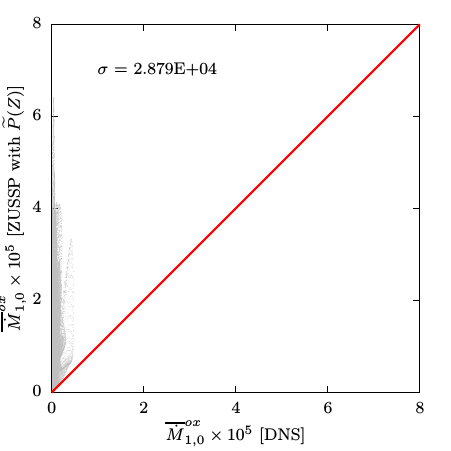
\includegraphics[width=\linewidth]{ch-subfiltermodeling/figures/lin-Mox4vsMox6-r3D-32}
    %\vspace{1ex}
  \end{subfigure}
  \begin{subfigure}[b]{0.375\linewidth}
    \centering
    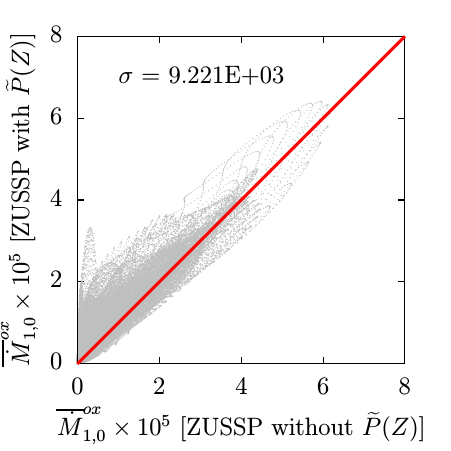
\includegraphics[width=\linewidth]{ch-subfiltermodeling/figures/lin-Mox4vsMox3-r3D-32}
  \end{subfigure}%%
  \begin{subfigure}[b]{0.375\linewidth}
    \centering
    \includegraphics[width=\linewidth]{ch-subfiltermodeling/figures/linear-cdf-ox-ZUSSP-r3D-32}
  \end{subfigure}
  \caption[Error Associated with $\pz = \beta(Z;\tf{Z},\tf{Z_V})$ for $\fst[M]{1,0}^{ox}$]{Filtered moment source term for oxidation [m$^3$/(s$\cdot$m$^3$)] at $t = 5$ ms evaluated with \cref{eq:subfilter:dns:mzusspwithoutpz,eq:subfilter:dns:mzusspwithpz,eq:subfilter:dns:mdns} for a normalized filter width of $\Delta/h = 32$. In the first three plots, the red lines represent a one-to-one correspondence and the sample standard deviation is indicated at the top left corner. In the fourth, bottom right plot, the solid red line is the ``DNS'' case, the cyan dashed line is the ``ZUSSP without $\pz$'' case, and the blue dashed line is the ``ZUSSP with $\pz$'' case.}
  \label{fig:subfilter:dns:erroronbetaox}
\end{figure}

Now that the form of $\pz$ has been confirmed, the filtered moment source term for oxidation using the $Z$-Activated Soot Subfilter PDF can be evaluated. The latter shall be referred to as the ``ZASSP with $\pz$'' case, and its expression is given by
\begin{equation}\label{eq:subfilter:dns:mzasspwithpz}
  \fst[M]{1,0}^{ox} = \frac{\int\limits_0^1 \{ k_{ox}(x_j)|Z(x_j) \}H(Z - Z_{st})\tf{P}(Z; \tf{Z}(x_j),\tf{Z_V}(x_j)) dZ}{\int\limits_0^1 H(Z - Z_{st})\tf{P}(Z; \tf{Z}(x_j),\tf{Z_V}(x_j)) dZ} \cdot \mean{M_{0,1}(x_j)}.
  % \fst[M]{1,0}^{ox} = \frac{\int\limits_0^1 \{ k_{ox}|Z \}H(Z - Z_{st})\pz dZ}{\int\limits_0^1 H(Z - Z_{st})\pz dZ} \cdot \mean{M_{0,1}(x_j)}.
\end{equation}

This case is plotted against the source term from DNS in \cref{fig:subfilter:dns:zasspcomparisonox}. In the left-hand plot, it is clear that the source term evaluated with the proposed model still overpredicts the oxidation rate when compared to the values from DNS. However, when contrasted with the top right plot of \cref{fig:subfilter:dns:erroronbetaox}, the magnitudes of the largest source terms are reduced by nearly half. A direct comparison between the source terms using the $Z$-Uniform and $Z$-Activated Soot Subfilter PDFs, available in the middle plot of \cref{fig:subfilter:dns:zasspcomparisonox}, demonstrates that the latter tends to produce smaller oxidation rates than the former. This is expected, for the $Z$-Activated Soot Subfilter PDF was formulated to eliminate the unphysical contributions to the oxidation rate that the $Z$-Uniform Soot Subfilter PDF possessed.

\begin{figure}[ht]
  \centering
  \begin{subfigure}[b]{0.33\linewidth}
    \centering
    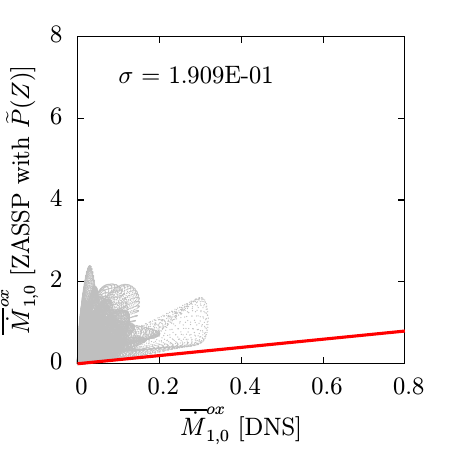
\includegraphics[width=\linewidth]{ch-subfiltermodeling/figures/lin-Mox5vsMox6-r3D-32}
  \end{subfigure}%%
  \begin{subfigure}[b]{0.33\linewidth}
    \centering
    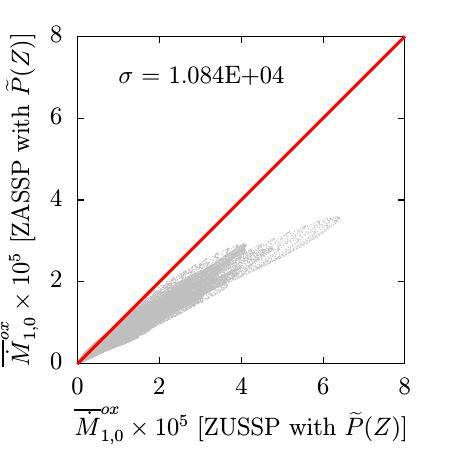
\includegraphics[width=\linewidth]{ch-subfiltermodeling/figures/lin-Mox5vsMox4-r3D-32}
  \end{subfigure}%%
  \begin{subfigure}[b]{0.33\linewidth}
    \centering
    \includegraphics[width=\linewidth]{ch-subfiltermodeling/figures/linear-cdf-ox-ZASSP-r3D-32}
  \end{subfigure}
  \caption[Comparison of ZASSP with $\pz$ to DNS \& ZUSSP with $\pz$ for $\fst[M]{1,0}^{ox}$]{Comparison of the ``ZASSP with $\pz$'' case to the ``DNS'' and ``ZUSSP with $\pz$'' cases for the same conditions as in \cref{fig:subfilter:dns:erroronbetaox}. In the right-hand plot, the solid red line is the ``DNS'' case, the blue dashed line is the ``ZUSSP with $\pz$'' case, and the magenta dashed line is the ``ZASSP with $\pz$'' case.}
  \label{fig:subfilter:dns:zasspcomparisonox}
\end{figure}

The CDF in the right-hand plot of \cref{fig:subfilter:dns:zasspcomparisonox} more clearly reveals the extent of the oxidation source term reduction. It is evident that the proposed model has a greater proportion of smaller source terms relative to the ``ZUSSP with $\pz$'' case, albeit the effect is not enough to replicate the CDF from the DNS. Nevertheless, the effectiveness of the proposed model is expected to increase with the filter width due to the expanded presence of lean subfilter regions, which is a consequence of the enlargened variance in mixture fraction. This point will be explored in \cref{sec:subfilter:dns:fw}. Additionally, a model modification that involves rich-shifting the activation location of the sooting mode is expected to further reduce the magnitudes of the oxidation source terms and will be presented in \cref{sec:conclusion:future:zassp}.


\subsection{Surface Growth Source Term}
\label{sec:subfilter:dns:sg}

The $Z$-Activated Soot Subfilter PDF of \cref{sec:subfilter:zassp} has demonstrated the ability to decrease the magnitude of the filtered moment source term for oxidation through the elimination of unphysical contributions at lean mixture fractions. On the other hand, its effect on the source terms for nucleation, condensation, and surface growth has not been investigated yet. These modes of soot evolution are sensitive to the flame structure, and surface growth by the HACA mechanism~\cite{frenklach1985,frenklach1991} can even be a prominent mode of soot growth in near-flame regions, leading to intensified interactions between soot and gas-phase chemistry. However, surface growth is confined to rich regions, so the $Z$-Activated Soot Subfilter PDF is not expected to strongly influence this source term. Confirmation of this hypothesis will be the focus of this subsection.

% Soot oxidation is certainly the dominant mode in these below-stoichiometric regions, but the filtered moment source terms for surface growth could potentially be nonzero, as extrapolation may suggest in \cref{fig:subfilter:leszussp:kvsz}.

% In near-flame regions, surface growth by the HACA mechanism~\cite{frenklach1985,frenklach1991} can be a prominent mode of soot growth and can lead to intensified interactions between soot and gas-phase chemistry. The $Z$-activated soot subfilter PDF was formulated to account for such interactions, so it is worthwhile to analyze its impact on this source term.

As for oxidation, this analysis will investigate the surface growth source term contribution to the total volume fraction, $\fst[M]{1,0}^{sg}$. The aptly named surface growth involves reactions on the soot surface, so the expression for the source term depends on the filtered moment for the total soot surface area $\mean{M}_{0,1}$. As before, the surface growth coefficient $k_{sg}(Z)$ is not present in the DNS database, so it will be taken with a density-weighted conditional average
\begin{equation}\label{eq:subfilter:dns:condksg}
  \begin{split}
    k_{sg}(Z) &\approx \{ k_{sg}(x_j)|Z(x_j) \} \\
    &= \frac{<\rho(x_j)k_{sg}(x_j)|Z(x_j)>}{<\rho(x_j)|Z(x_j)>}.
  \end{split}
\end{equation}
This quantity is plotted in \cref{fig:subfilter:dns:ksg}. The scatter is relatively larger than that of the oxidation coefficient, as expected from \cref{fig:subfilter:leszussp:kvsz}, but, again, modeling of the subfilter PDF is the primary concern here.

%, where it is evident that the surface growth coefficient at mixture fractions $Z < 0.2$ and $Z > 0.4$ is modeled well by \cref{eq:subfilter:dns:condksg}. However, in a similar observation as before, the large spread of the DNS field in $0.2 < Z < 0.4$ indicates that additional conditional averaging against the scalar dissipation rate or another variable could provide a more accurate approximation.

\begin{figure}[htb]
  \centering
  \includegraphics[width=0.43\linewidth]{ch-subfiltermodeling/figures/ksgvsz}
  \caption[Approximation for Surface Growth Coefficient, $k_{sg}(Z)$]{Density-weighted, conditionally averaged approximation for the surface growth coefficient $k_{sg}(Z)$. All symbols and lines are analogous to those in \cref{fig:subfilter:dns:kox}.}
  \label{fig:subfilter:dns:ksg}
\end{figure}

The subfilter PDF for mixture fraction $\pz$ needs to be modeled as well, and the form of a beta distribution will be presumed. The error associated with this presumption is quantified in \cref{fig:subfilter:dns:erroronbetasg}, where the bottom left plot shows the standard deviation is nearly half of that associated with the form of the soot subfilter PDF (top two plots). The CDF in the bottom right plot reveals that the distance between the lines representing \cref{eq:subfilter:dns:mzusspwithoutpz,eq:subfilter:dns:mzusspwithpz} (adapted for surface growth) is generally less than the distance between the latter and the source term from DNS. Note that the difference between the two errors is not as dramatic as in the CDF from \cref{fig:subfilter:dns:erroronbetaox} for oxidation. Nevertheless, the error associated with presuming the form of a beta distribution for $\pz$ is relatively small for most values of $\fst[M]{1,0}^{sg}$.

% In fact, even at intermediate values of $\fst[M]{1,0}^{sg}$, the error from presuming a beta distribution is comparable to that from the choice of the soot subfilter PDF. Nonetheless, the largest source terms are the most important for this \textit{a priori} analysis as they correspond to heavy growth in the slightly rich, near-flame regions. For these values, the error associated with presuming the form of a beta distribution for $\pz$ is relatively small.

\begin{figure}[ht]
  \centering
  \begin{subfigure}[b]{0.375\linewidth}
    \centering
    \includegraphics[width=\linewidth]{ch-subfiltermodeling/figures/lin-Msg3vsMsg6-r3D-32}
    %\vspace{1ex}
  \end{subfigure}%%
  \begin{subfigure}[b]{0.375\linewidth}
    \centering
    \includegraphics[width=\linewidth]{ch-subfiltermodeling/figures/lin-Msg4vsMsg6-r3D-32}
    %\vspace{1ex}
  \end{subfigure}
  \begin{subfigure}[b]{0.375\linewidth}
    \centering
    \includegraphics[width=\linewidth]{ch-subfiltermodeling/figures/lin-Msg4vsMsg3-r3D-32}
  \end{subfigure}%%
  \begin{subfigure}[b]{0.375\linewidth}
    \centering
    \includegraphics[width=\linewidth]{ch-subfiltermodeling/figures/linear-cdf-sg-ZUSSP-r3D-32}
  \end{subfigure}
  \caption[Error Associated with $\pz = \beta(Z;\tf{Z},\tf{Z_V})$ for $\fst[M]{1,0}^{sg}$]{Filtered moment source term for surface growth [m$^3$/(s$\cdot$m$^3$)] at the same conditions of \cref{fig:subfilter:dns:erroronbetaox}. All symbols and lines are analogous to those in \cref{fig:subfilter:dns:erroronbetaox}.}
  \label{fig:subfilter:dns:erroronbetasg}
\end{figure}

The filtered moment source term for surface growth using the $Z$-Activated Soot Subfilter PDF can now be evaluated using an expression analogous to \cref{eq:subfilter:dns:mzasspwithpz}. This case is plotted against the source term from DNS in \cref{fig:subfilter:dns:zasspcomparisonsg}. When the left-hand image is compared to the top right image of \cref{fig:subfilter:dns:erroronbetasg}, the profiles of the source terms utilizing the $Z$-Uniform and $Z$-Activated Soot Subfilter PDFs are nearly identical. This finding indicates that use of the proposed model hardly affects the evaluation of the surface growth source term, which is further confirmed by the middle and right-hand plots of \cref{fig:subfilter:dns:zasspcomparisonsg}. Such a behavior is expected, for the $Z$-Activated Soot Subfilter PDF was formulated to eliminate any unphysical contributions from regions of lean mixture fraction. However, as shown in \cref{fig:subfilter:dns:ksg}, the surface growth coefficient in those regions is negligible. Almost no unphysical contributions exist, so the source term evaluated with the proposed model and the $Z$-Uniform Soot Subfilter PDF should be very similar.
%In the CDF plot of \cref{fig:subfilter:dns:zasspcomparisonsg}, it is also interesting to note that both soot subfilter PDFs tend to overpredict the largest surface growth source terms and underpredict the smallest when compared to the values from DNS.

\begin{figure}[ht]
  \centering
  \begin{subfigure}[b]{0.33\linewidth}
    \centering
    \includegraphics[width=\linewidth]{ch-subfiltermodeling/figures/lin-Msg5vsMsg6-r3D-32}
  \end{subfigure}%%
  \begin{subfigure}[b]{0.33\linewidth}
    \centering
    \includegraphics[width=\linewidth]{ch-subfiltermodeling/figures/lin-Msg5vsMsg4-r3D-32}
  \end{subfigure}%%
  \begin{subfigure}[b]{0.33\linewidth}
    \centering
    \includegraphics[width=\linewidth]{ch-subfiltermodeling/figures/linear-cdf-sg-ZASSP-r3D-32}
  \end{subfigure}
  \caption[Comparison of ZASSP with \texorpdfstring{$\pz$}{P(Z)} to DNS \& ZUSSP with \texorpdfstring{$\pz$}{P(Z)} for \texorpdfstring{$\fst[M]{1,0}^{sg}$}{M1,0sg}]{Comparison of the ``ZASSP with $\pz$'' case to the ``DNS'' and ``ZUSSP with $\pz$'' cases for the same conditions as in \cref{fig:subfilter:dns:erroronbetaox}. All symbols and lines are analogous to those in \cref{fig:subfilter:dns:zasspcomparisonox}.}
  \label{fig:subfilter:dns:zasspcomparisonsg}
\end{figure}


\subsection{Effects of Filter Width}
\label{sec:subfilter:dns:fw}

In grid-filtered LES, the computational expense is directly related to the resolution of the grid. A larger grid spacing reduces the cost but also elevates the cutoff for the length and time scales that need to be modeled. Therefore, it is important to analyze how the proposed model performs as the filter width is increased. As before, the filtered moment source terms for oxidation and surface growth, given by the analogous forms of \cref{eq:subfilter:dns:mzusspwithpz,eq:subfilter:dns:mzasspwithpz}, are the focus of this study. The estimates required for the oxidation and surface growth coefficients have already been investigated in \cref{sec:subfilter:dns:ox,sec:subfilter:dns:sg}, but the error associated with presuming a beta distribution for $\pz$ should be analyzed for an increasing normalized filter width $\Delta/h$. 

\begin{figure}[ht]
  \centering
  \begin{subfigure}[b]{0.33\linewidth}
    \centering
    \includegraphics[width=\linewidth]{ch-subfiltermodeling/figures/linear-cdf-ox-ZUSSP-r3D-4}
  \end{subfigure}%%
  \begin{subfigure}[b]{0.33\linewidth}
    \centering
    \includegraphics[width=\linewidth]{ch-subfiltermodeling/figures/linear-cdf-ox-ZUSSP-r3D-32}
  \end{subfigure}%%
  \begin{subfigure}[b]{0.33\linewidth}
    \centering
    \includegraphics[width=\linewidth]{ch-subfiltermodeling/figures/linear-cdf-ox-ZUSSP-r3D-128}
  \end{subfigure}
  \begin{subfigure}[b]{0.33\linewidth}
    \centering
    \includegraphics[width=\linewidth]{ch-subfiltermodeling/figures/linear-cdf-sg-ZUSSP-r3D-4}
  \end{subfigure}%%
  \begin{subfigure}[b]{0.33\linewidth}
    \centering
    \includegraphics[width=\linewidth]{ch-subfiltermodeling/figures/linear-cdf-sg-ZUSSP-r3D-32}
  \end{subfigure}%%
  \begin{subfigure}[b]{0.33\linewidth}
    \centering
    \includegraphics[width=\linewidth]{ch-subfiltermodeling/figures/linear-cdf-sg-ZUSSP-r3D-128}
  \end{subfigure}
  \caption[Error Associated with \texorpdfstring{$\pz = \beta(Z;\tf{Z},\tf{Z_V})$}{P(Z) = B(Z;Z,ZV)} for Various \texorpdfstring{$\Delta/h$}{D/h}]{CDFs of filtered moment source terms for oxidation (\textit{top}) and surface growth (\textit{bottom}) for normalized filter widths of $\Delta/h = 4$, 32, and 128 (\textit{left to right}). All lines are analogous to those in \cref{fig:subfilter:dns:erroronbetaox}.}
  \label{fig:subfilter:dns:erroronbetafwidth}
\end{figure}

The CDFs of the source terms for oxidation and surface growth are plotted in \cref{fig:subfilter:dns:erroronbetafwidth}. As expected, the ``ZUSSP without $\pz$'' and ``ZUSSP with $\pz$'' cases nearly collapse on the ``DNS'' case for a normalized filter width of 4. The filter width is small enough that presuming a beta distribution for $\pz$ does not have a significant impact on the source term. On the other hand, increasing the normalized filter width to 128 degrades the accuracy of the presumption, especially for the surface growth source term. Presuming a beta distribution may not be appropriate for all conditions, and another distribution may be needed for a more accurate depiction of the subfilter mixture fraction field at large filter widths. Determination of this distribution will be the subject of future work, but, for the remainder of this analysis, the beta distribution will be presumed.

The filtered moment source term for oxidation evaluated with \cref{eq:subfilter:dns:mzasspwithpz} is compared to the source term evaluated with \cref{eq:subfilter:dns:mzusspwithpz} in the top plots of \cref{fig:subfilter:dns:moxfwidth}. For a normalized filter width of 4, the former only slightly underpredicts the rate of oxidation compared to the latter. As the filter width is broadened, the proposed model decreases the oxidation rate more intensely. The CDFs confirm this trend, but the proposed model still overestimates the overall rate of oxidation when compared to the values from DNS.

\begin{figure}[ht]
  \centering
  \begin{subfigure}[b]{0.33\linewidth}
    \centering
    \includegraphics[width=\linewidth]{ch-subfiltermodeling/figures/lin-Mox5vsMox4-r3D-4}
  \end{subfigure}%%
  \begin{subfigure}[b]{0.33\linewidth}
    \centering
    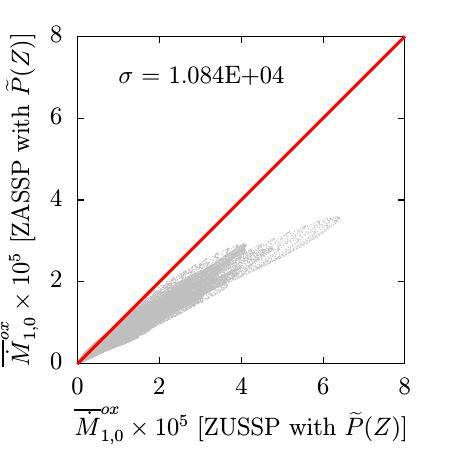
\includegraphics[width=\linewidth]{ch-subfiltermodeling/figures/lin-Mox5vsMox4-r3D-32}
  \end{subfigure}%%
  \begin{subfigure}[b]{0.33\linewidth}
    \centering
    \includegraphics[width=\linewidth]{ch-subfiltermodeling/figures/lin-Mox5vsMox4-r3D-128}
  \end{subfigure}
  %% \begin{subfigure}[b]{0.33\linewidth}
  %%   \centering
  %%   \includegraphics[width=\linewidth]{ch-subfiltermodeling/figures/lin-Mox5vsMox6-r3D-4}
  %% \end{subfigure}%%
  %% \begin{subfigure}[b]{0.33\linewidth}
  %%   \centering
  %%   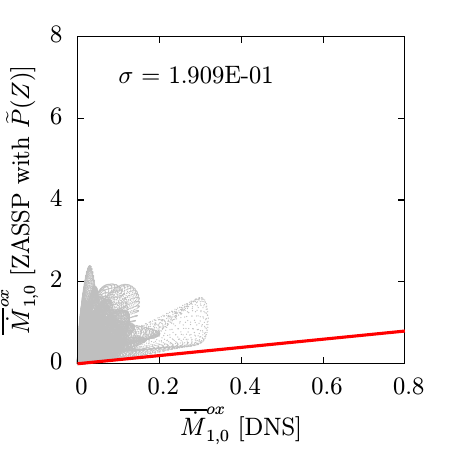
\includegraphics[width=\linewidth]{ch-subfiltermodeling/figures/lin-Mox5vsMox6-r3D-32}
  %% \end{subfigure}%%
  %% \begin{subfigure}[b]{0.33\linewidth}
  %%   \centering
  %%   \includegraphics[width=\linewidth]{ch-subfiltermodeling/figures/lin-Mox5vsMox6-r3D-128}
  %% \end{subfigure}
  \begin{subfigure}[b]{0.33\linewidth}
    \centering
    \includegraphics[width=\linewidth]{ch-subfiltermodeling/figures/linear-cdf-ox-ZASSP-r3D-4}
  \end{subfigure}%%
  \begin{subfigure}[b]{0.33\linewidth}
    \centering
    \includegraphics[width=\linewidth]{ch-subfiltermodeling/figures/linear-cdf-ox-ZASSP-r3D-32}
  \end{subfigure}%%
  \begin{subfigure}[b]{0.33\linewidth}
    \centering
    \includegraphics[width=\linewidth]{ch-subfiltermodeling/figures/linear-cdf-ox-ZASSP-r3D-128}
  \end{subfigure}
  \caption[\texorpdfstring{$\fst[M]{1,0}^{ox}$}{M1,0ox} Using ZASSP with $\pz$ for Various \texorpdfstring{$\Delta/h$}{D/h}]{\textit{Top} - Comparison of the ``ZASSP with $\pz$'' case to the ``ZUSSP with $\pz$'' case at $t = 5$ ms for the oxidation source term. \textit{Bottom} - CDFs of filtered moment source terms for oxidation using the ``ZASSP with $\pz$'' case. Lines for the bottom plots are analogous to those in \cref{fig:subfilter:dns:zasspcomparisonox}. \textit{Left to right} - Normalized filter widths of $\Delta/h = 4$, 32, and 128, respectively.}
  \label{fig:subfilter:dns:moxfwidth}
\end{figure}

The mixture fraction variance increases with the filter width, so the reduction in the oxidation source term can be explained by plotting the ratio of oxidation coefficients from \cref{eq:subfilter:zussp:ox,eq:subfilter:zassp:kox} as a function of the filtered mixture fraction variance. In \cref{fig:subfilter:dns:coeffvszvar}, a growing variance leads to a maximum fivefold reduction in the oxidation coefficient from the proposed model relative to the coefficient from the source term using the $Z$-Uniform Soot Subfilter PDF. %This property is likely the cause for the twofold reduction in the oxidation source term, as shown in the top plots of \cref{fig:subfilter:dns:moxfwidth}.

%% In the CDFs of \cref{fig:subfilter:dns:moxfwidth}, it is also notable that the proportion of source terms with larger values increases with the filter width. The presence of source terms with values greater than $10^3$ becomes dominant at the largest filter width of $\Delta/h = 128$. This suggests that more intense oxidation events occur.

\begin{figure}[htb]
  \centering
  \includegraphics[width=0.43\linewidth]{ch-subfiltermodeling/figures/oxcoeffvszvar-chi10-C7H16}
  \caption[Ratio of Oxidation Coefficients vs. \texorpdfstring{$\tf{Z_{\text{V}}}$}{Zv}]{Ratio of oxidation coefficients versus mixture fraction variance from a flamelet solution for the same nitrogen-diluted, \textit{n}-heptane mixture at $\chi_{st} = 10$ s$^{-1}$. $\tf{k}_{ox}$ is given in \cref{eq:subfilter:zussp:ox}, and $\check{k}_{ox}$ is given in \cref{eq:subfilter:zassp:kox}.}
  \label{fig:subfilter:dns:coeffvszvar}
\end{figure}

The filtered moment source term for surface growth evaluated with the analogous form of \cref{eq:subfilter:dns:mzasspwithpz} is juxtaposed with the analogous source term from \cref{eq:subfilter:dns:mzusspwithpz} in the top plots of \cref{fig:subfilter:dns:msgfwidth}. Although the proposed model overestimates the magnitude of the surface growth rate compared to the source term with the $Z$-Uniform Soot Subfilter PDF, the standard deviations normalized by the maximum source term magnitudes are much less than those of \cref{fig:subfilter:dns:moxfwidth}. Expanding the filter width does not drastically increase the difference between the source terms of \cref{eq:subfilter:dns:mzasspwithpz,eq:subfilter:dns:mzusspwithpz}. This trend agrees with the analysis from \cref{fig:subfilter:dns:zasspcomparisonsg}, where it was found that use of the proposed model hardly affects the evaluation of the surface growth source term. % These observations are especially relevant at the largest values of the surface growth rate even as the filter width is broadened, as shown in the CDF plots of \cref{fig:subfilter:dns:msgfwidth}.

\begin{figure}[ht]
  \centering
  \begin{subfigure}[b]{0.33\linewidth}
    \centering
    \includegraphics[width=\linewidth]{ch-subfiltermodeling/figures/lin-Msg5vsMsg4-r3D-4}
  \end{subfigure}%%
  \begin{subfigure}[b]{0.33\linewidth}
    \centering
    \includegraphics[width=\linewidth]{ch-subfiltermodeling/figures/lin-Msg5vsMsg4-r3D-32}
  \end{subfigure}%%
  \begin{subfigure}[b]{0.33\linewidth}
    \centering
    \includegraphics[width=\linewidth]{ch-subfiltermodeling/figures/lin-Msg5vsMsg4-r3D-128}
  \end{subfigure}
  \begin{subfigure}[b]{0.33\linewidth}
    \centering
    \includegraphics[width=\linewidth]{ch-subfiltermodeling/figures/linear-cdf-sg-ZASSP-r3D-4}
  \end{subfigure}%%
  \begin{subfigure}[b]{0.33\linewidth}
    \centering
    \includegraphics[width=\linewidth]{ch-subfiltermodeling/figures/linear-cdf-sg-ZASSP-r3D-32}
  \end{subfigure}%%
  \begin{subfigure}[b]{0.33\linewidth}
    \centering
    \includegraphics[width=\linewidth]{ch-subfiltermodeling/figures/linear-cdf-sg-ZASSP-r3D-128}
  \end{subfigure}
  \caption[\texorpdfstring{$\fst[M]{1,0}^{sg}$}{M1,0sg} Using ZASSP with $\pz$ for Various \texorpdfstring{$\Delta/h$}{D/h}]{\textit{Top} - Comparison of the ``ZASSP with $\pz$'' case to the ``ZUSSP with $\pz$'' case at $t = 5$ ms for the surface growth source term. \textit{Bottom} - CDFs of filtered moment source terms for surface growth using the ``ZASSP with $\pz$'' case. Lines for the bottom plots are analogous to those in \cref{fig:subfilter:dns:zasspcomparisonox}. \textit{Left to right} - Normalized filter widths of $\Delta/h = 4$, 32, and 128, respectively.}
  \label{fig:subfilter:dns:msgfwidth}
\end{figure}
